\begin{mychapter}{Presentazione del Progetto}

\begin{mysection}{Descrizione Generale}
Scalamarket è una moderna piattaforma e-commerce basata su un'architettura a microservizi, progettata per garantire elevata scalabilità, affidabilità e flessibilità. Il sistema gestisce l'intero ciclo di vita dell'acquisto online: dalla registrazione degli utenti, alla consultazione del catalogo, fino all'elaborazione degli ordini e alla gestione logistica delle spedizioni. L'intera infrastruttura è stata ideata per essere distribuita in modo efficiente tramite Kubernetes ed eventualmente ospitata in ambiente cloud AWS, fornendo un backend solido, scalabile e supportato da API RESTful. 


\begin{figure}[h]
    \centering
    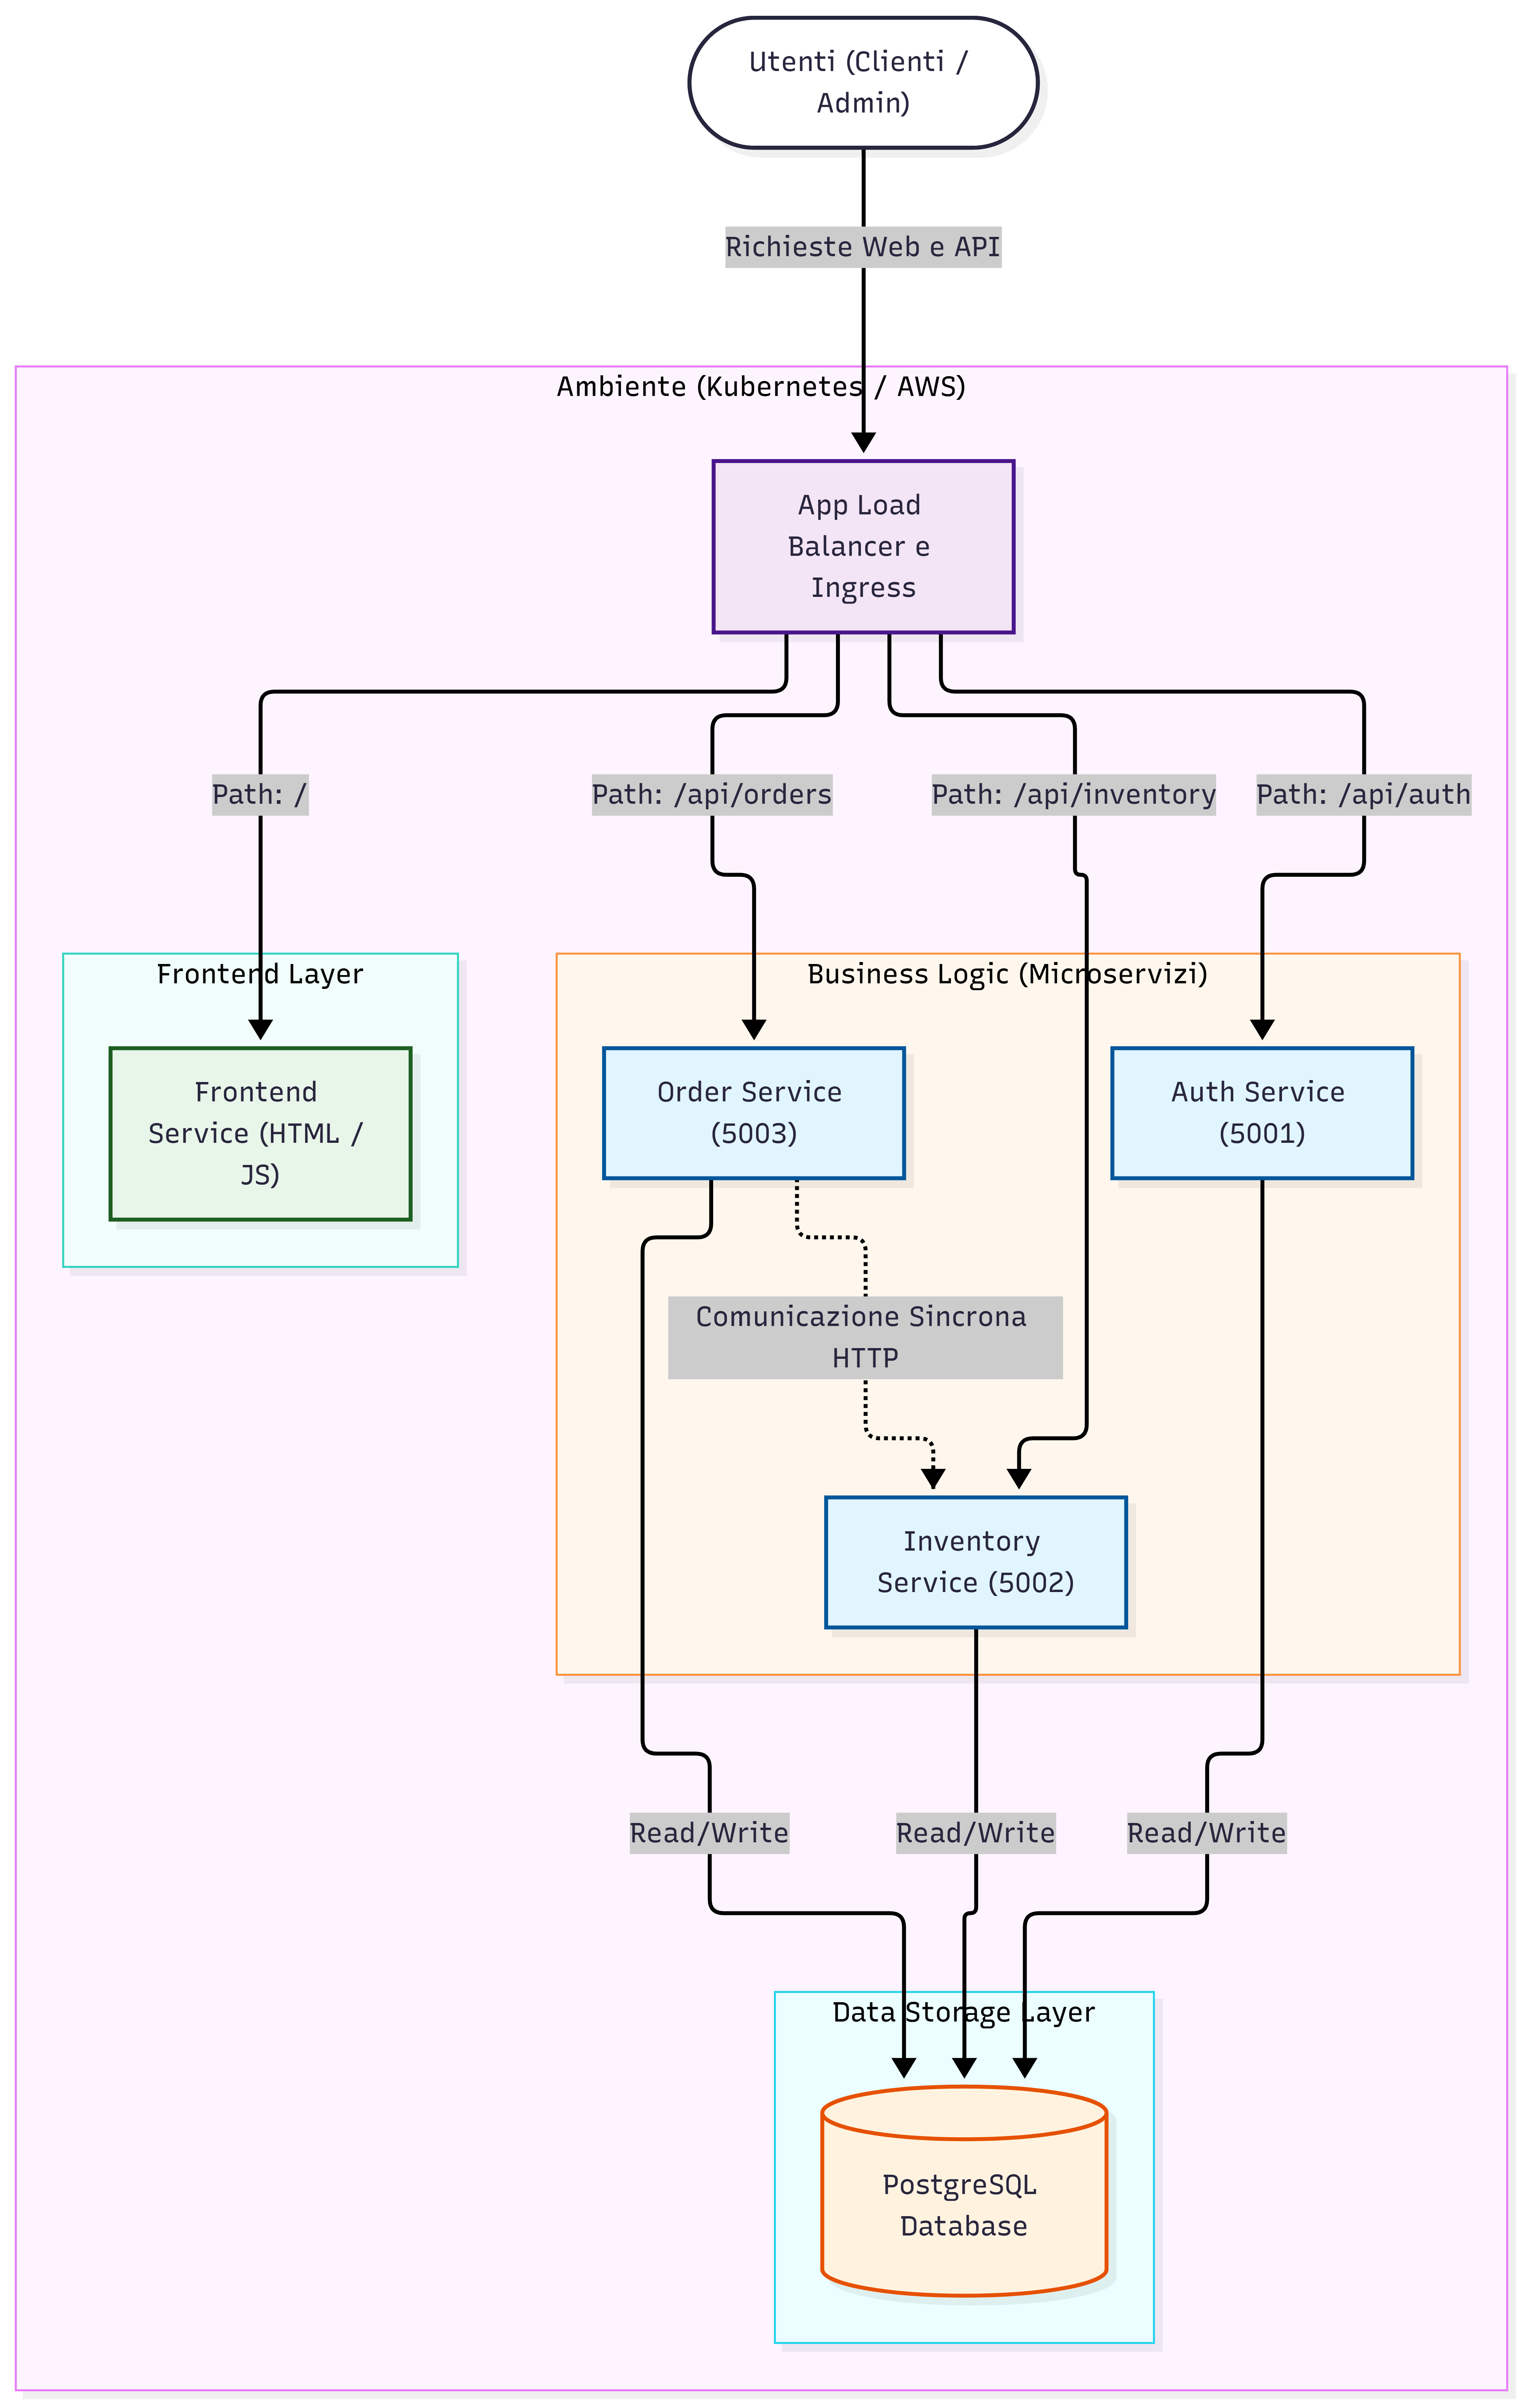
\includegraphics[width=\textwidth,height=0.45\textheight,keepaspectratio]{img/ComponentDiagram.png}
    \caption{Diagramma dei Componenti UML}
    \label{fig:component_diagram}
\end{figure}
\end{mysection}

\begin{mysection}{Requisiti dell'Applicativo}
L'applicativo è stato sviluppato per soddisfare i seguenti requisiti architetturali, funzionali e di business 

\begin{itemize}
    \item \textbf{Autenticazione e Autorizzazione (Auth Service):} Il sistema deve permettere la registrazione e il login sicuri sia per i clienti (Client) che per gli amministratori (Admin). L'amministratore deve avere i privilegi per gestire le utenze.
    \item \textbf{Gestione Inventario (Inventory Service):} Il sistema deve gestire un catalogo dinamico di articoli, tenendo traccia delle quantità ripartite in molteplici filiali. Deve inoltre impedire la creazione di ordini per articoli non disponibili.
    \item \textbf{Gestione Ordini e Logistica (Order Service):} L'applicativo deve processare il carrello dell'utente, allocando in tempo reale i prodotti necessari e scalandoli in modo intelligente dalle filiali che ne hanno disponibilità. Deve inoltre tracciare l'occupazione dei mezzi logistici, gestendo i furgoni in uso e quelli a disposizione.
    \item \textbf{Architettura a Microservizi e Dati Isolati:} Per massimizzare la modularità, ogni servizio deve possedere una propria logica di business e interfacciarsi con il proprio database PostgreSQL indipendente, disaccoppiando così i domini applicativi.
\end{itemize}

È importante specificare che l'applicativo è da considerarsi un Prototipo (Proof of Concept) atto a dimostrare le dinamiche di scalabilità, distribuzione e interazione tra microservizi, e non è pensato per un utilizzo commerciale in produzione. Alcune interfacce, così come la maggior parte delle funzionalità di sicurezza sono da considerarsi basilari

\begin{figure}[h]
    \centering
    \includegraphics[width=\textwidth,height=0.45\textheight,keepaspectratio]{img/SequenceDiagram.png}
    \caption{Diagramma di Sequenza}
    \label{fig:sequence_diagram}
\end{figure}

\end{mysection}

\begin{mysection}{Il Sito Web}
Per l'implementazione di Scalamarket si è scelto un framework Flask. Il lato client e il pannello di gestione amministrativa sono stati realizzati mediante un'interfaccia web responsive integrata con il backend. L'applicazione espone e gestisce tutti gli endpoint necessari, mentre la UI comunica costantemente con questi servizi tramite chiamate asincrone.

Il sito implementa tre diverse interfacce: \textbf{Cliente}, \textbf{Gestore Filiale} ed \textbf{Amministratore Globale}.

\begin{itemize}
    \item \textbf{Interfaccia Cliente:} L'utente può scorrere l'intero catalogo, visualizzare i prezzi e le disponibilità massime, aggiungere elementi al carrello e, una volta inviato l'ordine, monitorarne lo stato e i dettagli dei prodotti tramite un'apposita cronologia.
    \item \textbf{Interfaccia Amministratore Globale:} L'admin ha accesso a una dashboard completa che gli permette di visualizzare l'inventario globale (con possibilità di ricerca rapida), controllare in tempo reale lo stato logistico totale, visionare ed eliminare lo storico ordini globale e monitorare/eliminare gli account utenti.
    \item \textbf{Interfaccia Gestore Filiale:} Il gestore ha una visione limitata esclusivamente alle giacenze e ai veicoli della propria sede, con i poteri esclusivi di poter aggiungere o rimuovere articoli dal catalogo, e aggiornare le scorte e i mezzi assegnati alla filiale.
\end{itemize}

\textit{Nota: per un'analisi dettagliata e visiva di come è strutturata l'interfaccia utente (UI) nelle sue varie schermate, si rimanda al quinto capitolo, "Interfaccia Utente", del documento.}

\begin{figure}[h]
    \centering
    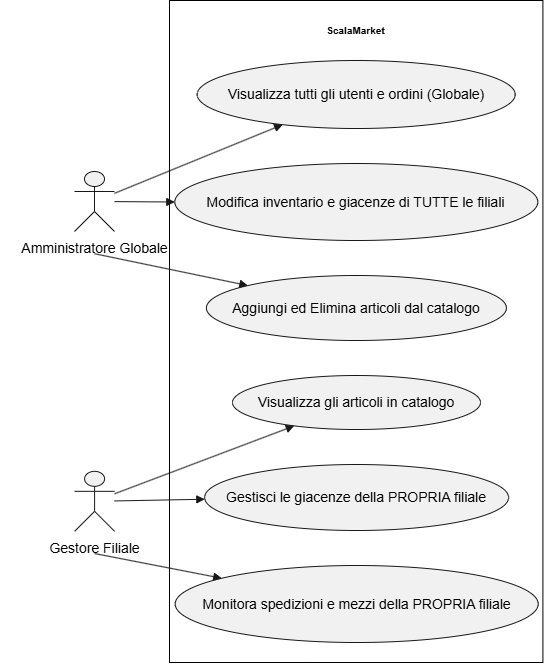
\includegraphics[width=\textwidth,height=0.45\textheight,keepaspectratio]{img/UseCaseDiagram.png}
    \caption{Diagramma dei Casi d'Uso}
    \label{fig:use_case_diagram}
\end{figure}

\end{mysection}

\end{mychapter}

\begin{mychapter}{Orchestrazione Kubernetes}

\begin{mysection}{Infrastruttura del Cluster}
L'infrastruttura Kubernetes poggia su componenti isolati al fine di scalare singolarmente in base alle esigenze e prevenire disservizi totali (\textit{Single Point of Failure}). 

I componenti base dell'applicativo sono i seguenti:
\begin{itemize}
    \item \textbf{frontend} (nginx): Gestisce la GUI per clienti e amministratori, esposto sulla porta 8080.
    \item \textbf{auth-service} (Flask): Gestisce autenticazione, registrazione e ruoli.
    \item \textbf{inventory-service} (Flask): Gestisce il catalogo, articoli e giacenze.
    \item \textbf{order-service} (Flask): Gestisce gli ordini, lo storico e la logistica.
    \item \textbf{postgres}: Database centrale con storage persistente garantito da un \texttt{PersistentVolume} (PV) e un \texttt{PersistentVolumeClaim} (PVC), logicamente frammentato in 3 database separati.
\end{itemize}

\subsubsection*{Ridondanza e Scalabilità}
I servizi stateless (Frontend e Logica di Business) sono stati configurati con repliche multiple, distribuite automaticamente dal \texttt{Service} \texttt{ClusterIP} che funge da load-balancer interno:
\begin{itemize}
    \item \textbf{Frontend (nginx):} 2 repliche per garantire alta disponibilità durante aggiornamenti o guasti di un Pod.
    \item \textbf{Logica di Business (auth, inventory, order):} 3 repliche ciascuno, in quanto soggetti a maggior stress e richieste concorrenti (es. elaborazione parallela ordini o scritture simultanee inventario).
    \item \textbf{Database (postgres):} Rimane a 1 replica. In ambiente nativo relazionale, la coerenza dei dati orizzontale richiede approcci dedicati; mantenere 1 replica ne previene il partizionamento anomalo.
\end{itemize}

Tutti i container Flask sono inoltre dotati di \texttt{resources} (requests e limits) per evitare che un consumo anomalo da parte di un Pod degradi le prestazioni degli altri (\textit{noisy neighbor}).

\subsubsection*{Kubernetes Ingress Controller}
L'accesso esterno e il routing dei servizi avvengono tramite un \textbf{Kubernetes Ingress Controller} (basato su NGINX) che agisce da \textit{reverse proxy} HTTP a livello di cluster. Attraverso un unico indirizzo esposto al pubblico, elimina la necessità di port-forward multipli. Le rotte principali implementate sono:
\begin{itemize}
    \item \texttt{/} $\rightarrow$ \texttt{frontend-service:8080}
    \item \texttt{/api/auth/} $\rightarrow$ \texttt{auth-service:5001}
    \item \texttt{/api/inventory/} $\rightarrow$ \texttt{inventory-service:5002}
    \item \texttt{/api/orders/} $\rightarrow$ \texttt{order-service:5003}
\end{itemize}

\textit{Nota: Si rimanda al quarto capitolo per un analisi più dettagliata delle rotte implementate e quali richieste vengono gestite da ciascuna di esse.}

\subsubsection*{Analisi dei Manifest Kubernetes}
L'architettura descritta è governata da una serie di manifest Kubernetes (file YAML) che dichiarano in maniera esplicita lo stato desiderato dell'infrastruttura.

\begin{itemize}
    \item \textbf{Ingress Locale (\texttt{ingress-local.yaml}):} Definisce le regole di instradamento specificando la \textit{ingressClassName} \texttt{nginx}. La risorsa si suddivide in blocchi \texttt{rules} che incanalano le chiamate ai backend giusti.
    \item \textbf{Deployment di un Microservizio (es. \texttt{order-deployment.yaml}):} Illustra le \textit{best-practice} del deployment stateless in Kubernetes. Specifica \texttt{replicas: 3}, \texttt{imagePullPolicy} e l'iniezione delle \texttt{env} necessarie (come la stringa di connessione DB). Impone infine limiti rigidi sulle \texttt{resources.requests} e \texttt{resources.limits} di CPU/RAM.
    \item \textbf{Deployment del Database (\texttt{postgres-deployment.yaml}):} A differenza dei precedenti, usa i \textit{Volumes}. Integra \texttt{volumeMounts} per i dati nel path \texttt{/var/lib/postgresql/data} collegati a un PVC. Inietta inoltre un \texttt{ConfigMap} nel path \texttt{/docker-entrypoint-initdb.d} per creare i database automaticamente all'avvio.
\end{itemize}

Di seguito viene riportato l'output dell'ambiente locale in esecuzione, che conferma lo stato \texttt{Running} di tutti i pod e la corretta visualizzazione della piattaforma dal browser locale.
\end{mysection}

\begin{figure}[H]
    \centering
    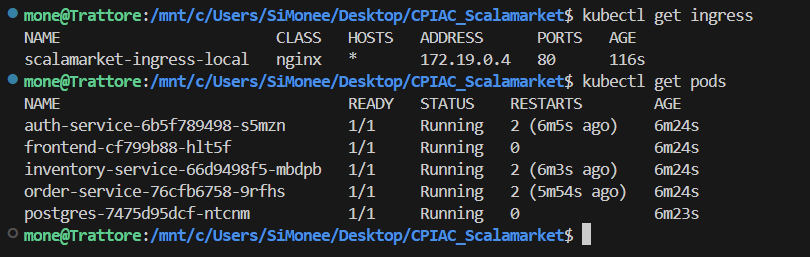
\includegraphics[width=\textwidth]{img/kubectl_local.png}
    \caption{Output del comando \texttt{kubectl get pods} nell'ambiente locale}
    \label{fig:kubectl_local}
\end{figure}

\begin{figure}[H]
    \centering
    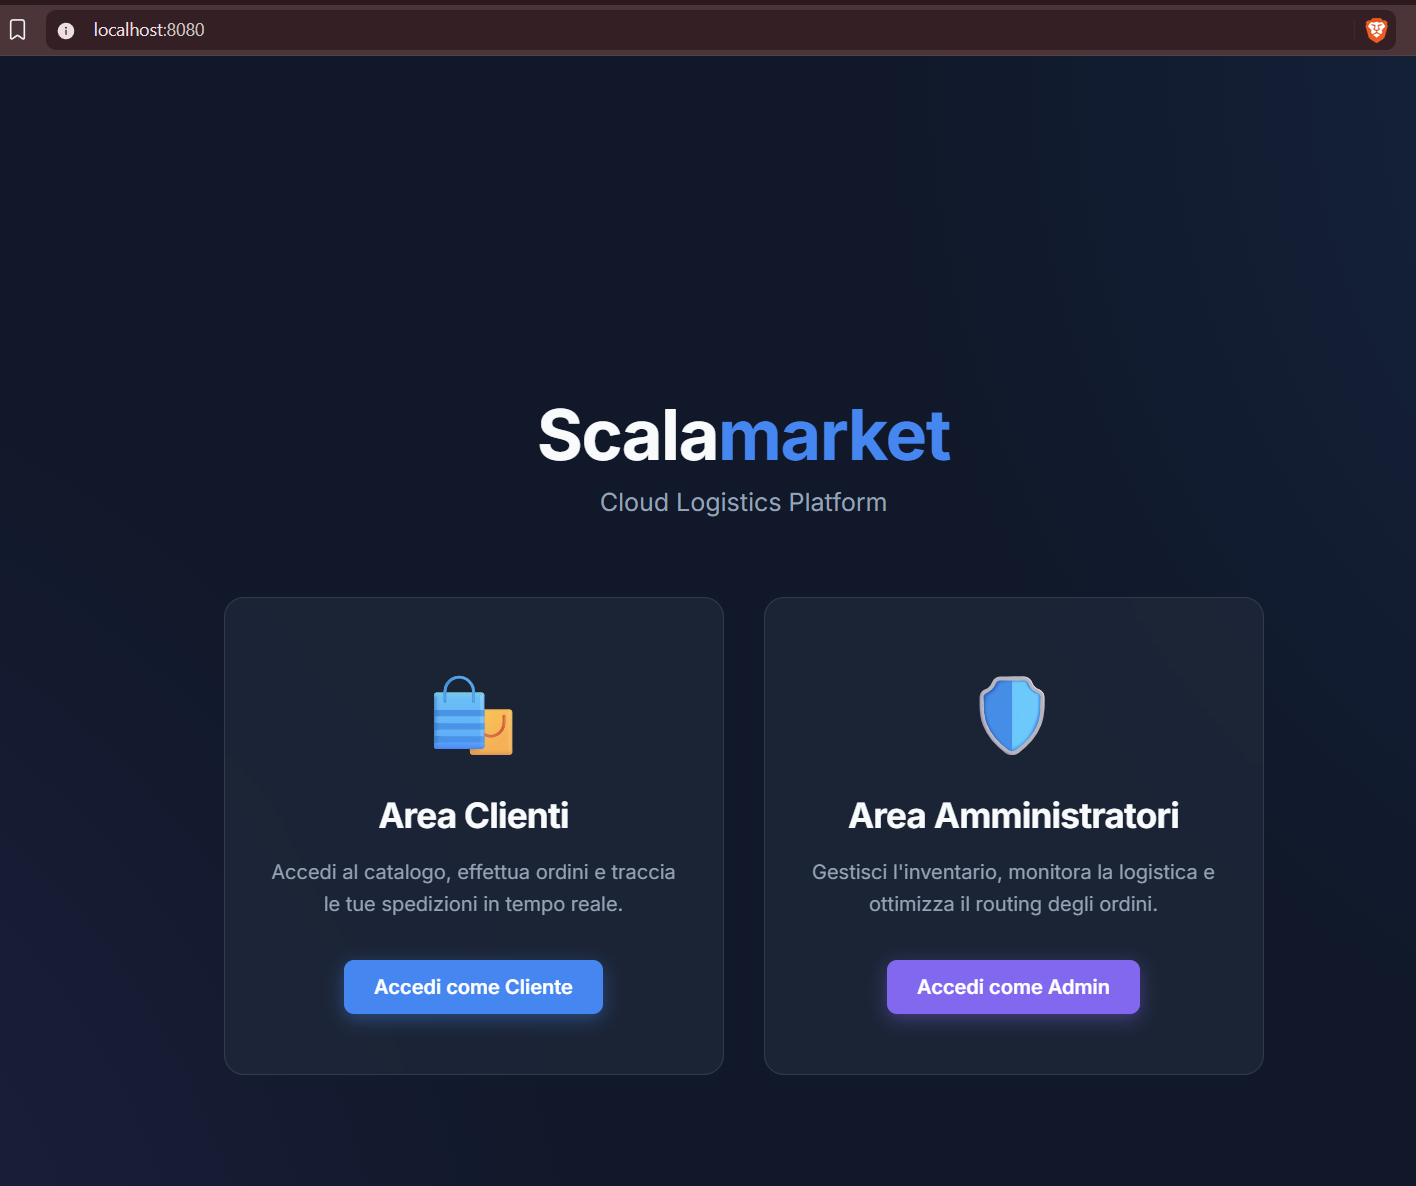
\includegraphics[width=\textwidth]{img/local_deployment.png}
    \caption{Piattaforma correttamente avviata ed esposta tramite localhost}
    \label{fig:local_deployment}
\end{figure}




\end{mychapter}

